
\documentclass[11pt,a4paper]{article}
\usepackage[utf8]{inputenc}
\usepackage[T1]{fontenc}
\usepackage{kotex}
\usepackage{geometry}
\usepackage{amsmath,amssymb}
\usepackage{siunitx}
\usepackage{booktabs,longtable}
\usepackage{graphicx}
\usepackage[dvipsnames]{xcolor}
\usepackage{hyperref}
\usepackage[nameinlink,capitalise]{cleveref}
\usepackage{enumitem}
\usepackage{titlesec}
\usepackage{listings}
\usepackage{caption}
\usepackage{subcaption}

\geometry{margin=1in}
\hypersetup{
    colorlinks=true,
    linkcolor=MidnightBlue,
    citecolor=RoyalBlue,
    urlcolor=RoyalBlue
}
\setlist[itemize]{topsep=2pt,itemsep=2pt,parsep=0pt,partopsep=0pt}
\setlist[enumerate]{topsep=2pt,itemsep=2pt,parsep=0pt,partopsep=0pt}

\titleformat{\section}{\large\bfseries}{\thesection}{0.5em}{}
\titleformat{\subsection}{\normalsize\bfseries}{\thesubsection}{0.5em}{}

\title{\textbf{RocksDB Put-Rate Model (Rewritten)\\
\large A Coherent Derivation with Added Explanations and Validation Plan}}
\author{Rewritten from \texttt{PutModel.html} with clarifying commentary}
\date{\today}

\begin{document}
\maketitle

\begin{abstract}
본 문서는 \texttt{PutModel.html}에 제시된 RocksDB 쓰기 경로 모델을 바탕으로,
논리적 일관성과 자연스러운 흐름에 초점을 맞추어 재구성한 LaTeX 문서이다.
핵심 기여는 (i) 기호/단위 표의 명시, (ii) \emph{장치 I/O 예산}과 \emph{증폭 계수}의
원인--결과 사슬 정리, (iii) \(\,S_{\max}\) (지속 가능한 최대 put rate)의 도출을
제약식 수준에서 \emph{명확한 최소화(min)} 문제로 정식화, (iv) 레벨별 \emph{mass-balance}
관점의 읽기--쓰기 결합(coupling) 설명, (v) 과도(Transient)~\(\rightarrow\)~정상(Steady) 전이의
측정상 주의점, (vi) 체계적인 검증 절차와 성공 기준의 명문화이다.
실무 운용을 위한 튜닝 체크리스트와 한계/확장 논의도 포함한다.
\end{abstract}

\section{문서 개요와 문제 정의}
RocksDB의 쓰기 경로는 \emph{WAL}(\textit{Write-Ahead Log}) 기록, \emph{memtable} 플러시,
그리고 \emph{compaction}으로 구성된다.
사용자가 주입하는 유저 바이트 유량을 \(S\) (\si{B/s})라 할 때,
장치는 이 쓰기들이 유발하는 실제 \emph{디바이스 쓰기} \(W(S)\)와
\emph{디바이스 읽기} \(R(S)\)를 \emph{동시에} 감당해야 한다.
본 모델의 목표는 장치의 I/O 예산 하에서 \emph{지속 가능한 최대 put rate} \(S_{\max}\)를 계산하고,
레벨별로 \(W\)와 \(R\)의 기여도를 분해하여 병목과 튜닝 포인트를 파악하는 것이다.

\subsection{핵심 아이디어 (요약)}
\begin{itemize}
  \item \textbf{자원 상한(Constraints)}: 장치가 제공하는 쓰기/읽기/혼합 유효대역을
  \(B_w\), \(B_r\), \(B_{\text{eff}}\)로 표준화한다.
  \item \textbf{증폭 계수(Amplification)}: 압축률 \(CR\) (\(0{<}CR{\le}1\))과
  쓰기 앰플리피케이션 \(WA\) (\(WA{\ge}1\))가 유저 바이트를 디바이스 쓰기량으로 확대한다.
  \item \textbf{결합(Coupling)}: 레벨드(Leveled) 컴팩션에서 \emph{상위 레벨 쓰기}는
  \emph{하위 레벨 읽기}를 유발한다. 따라서 \(W(S)\), \(R(S)\)는 서로 독립이 아니다.
  \item \textbf{정식화}: 제약식 \(\{W\le B_w,\,R\le B_r,\,W{+}R\le B_{\text{eff}}\}\)을 만족하는
  \(S\) 중 최댓값을 \(S_{\max}\)로 둔다. 즉,
  \(\displaystyle S_{\max}=\min\{S_w,S_r,S_m\}\) 꼴로 계산된다.
\end{itemize}

\section{기호와 단위 (Notation)}
본 문서에서 사용하는 주요 기호와 단위는 \ref{tab:notation}과 같다.
필요시 ops/s로의 변환식도 제공한다.

\begin{longtable}{@{}l l p{0.57\linewidth}@{}}
    \caption{기호/단위 표}\label{tab:notation}\\
    \toprule
    기호 & 단위 & 정의 \\\midrule
    \endfirsthead
    \toprule
    기호 & 단위 & 정의 \\\midrule
    \endhead
    \(S\) & \si{B/s} & 유저가 주입하는 바이트 유량(put 바이트/초). 값/키 평균 크기로 ops/s로 변환 가능. \\
    \(B_w\) & \si{B/s} & 장치의 \textbf{쓰기} 지속 대역(예: fio \texttt{write.job} 측정). \\
    \(B_r\) & \si{B/s} & 장치의 \textbf{읽기} 지속 대역(예: fio \texttt{read.job} 측정). \\
    \(B_{\text{eff}}\) & \si{B/s} & 혼합 부하에서의 \textbf{유효} 지속 대역(예: fio \texttt{mix50.job}). \\
    \(CR\) & --- & 압축률(작을수록 더 잘 압축됨). 디바이스에 쓰이는 바이트는 \(S/CR\)에 비례. \\
    \(WA\) & --- & 쓰기 앰플리피케이션(LSM/레벨 병합으로 인한 재기록 포함). \(WA\ge1\). \\
    \(RA_c\) & --- & \emph{컴팩션 기인} 읽기 앰플리피케이션(서비스 읽기 제외). \\
    \(W(S)\) & \si{B/s} & 디바이스에서 발생하는 총 쓰기량. 보통 \(\frac{S}{CR}\cdot WA\)로 근사. \\
    \(R(S)\) & \si{B/s} & 디바이스에서 발생하는 총 읽기량. 보통 \(\frac{S}{CR}\cdot RA_c\)로 근사. \\
    \(\alpha_i,\beta_i\) & --- & 레벨 \(i\)의 쓰기/읽기 계수(\(\sum_i\alpha_i{=}WA,\;\sum_i\beta_i{=}RA_c\)). \\
    \bottomrule
\end{longtable}

\paragraph{ops/s 변환} 평균 값 크기를 \(\bar v\) (\si{B/op})라 하면
\(\,S_{\text{ops}}=\frac{S}{\bar v}\,\)로 변환한다.
키 크기/메타데이터 오버헤드는 상황에 따라 \(\bar v\)에 포함하거나 별도 항으로 둔다.

\section{가정과 모델 구성}
\subsection{컴팩션 스타일과 스코프}
기본 스코프는 \textbf{Leveled Compaction}이다. Universal/FIFO/TTL 등 변형은
부록에서 간단 코멘트로 다룬다. 대부분의 식은 \(WA\), \(RA_c\)의 \emph{측정 또는 보정} 값을
매개변수로 사용하므로 스타일 간 비교도 가능하다.

\subsection{장치 I/O 예산 (Calibration)}
실제 장치에서 지속 가능 대역을 다음과 같이 계측한다.
\begin{itemize}
  \item \(B_w\): 순수 쓰기 지속 대역 (fio \texttt{write.job}).
  \item \(B_r\): 순수 읽기 지속 대역 (fio \texttt{read.job}).
  \item \(B_{\text{eff}}\): 읽기/쓰기 혼재 시 유효 대역 (fio \texttt{mix50.job}).
\end{itemize}
혼합 간섭을 별도로 두는 이유는, 현장에서는 \emph{동시성 간섭}이 크기 때문이다.
\(B_{\text{eff}}\)는 보수적 상한을 제공한다.

\subsection{증폭 계수와 레벨 결합}
유저 바이트 \(S\)는 압축률 \(CR\)에 의해 \(\frac{S}{CR}\)으로 확대되어 디바이스에 기록될 잠재량이 된다.
레벨드 병합으로 인한 재기록이 더해져 \emph{총 쓰기량}은
\begin{equation}
  W(S) \;\approx\; \frac{S}{CR}\cdot WA
  \label{eq:W}
\end{equation}
으로 근사한다. 한편 레벨 결합(coupling)으로 인해 \emph{총 읽기량}은
\begin{equation}
  R(S) \;\approx\; \frac{S}{CR}\cdot RA_c,
  \label{eq:R}
\end{equation}
여기서 \(RA_c\)는 \emph{서비스 읽기}를 제외한 \emph{컴팩션 기인} 읽기 앰플리피케이션이다.
보다 세밀하게는 레벨 \(i\)의 계수 \(\alpha_i,\beta_i\)로
\(W=\tfrac{S}{CR}\sum_i \alpha_i\), \(R=\tfrac{S}{CR}\sum_i \beta_i\)로 쪼갠다.

\section{제약식과 \(S_{\max}\) 도출}
장치가 지속 운전 가능한 조건은 다음 \emph{동시 제약}을 만족하는 \(S\)의 집합이다.
\begin{align}
    &\text{(W)}\quad W(S)\le B_w, \label{c:w}\\
    &\text{(R)}\quad R(S)\le B_r, \label{c:r}\\
    &\text{(M)}\quad W(S)+R(S)\le B_{\text{eff}}. \label{c:m}
\end{align}
\cref{eq:W,eq:R}를 대입하면 각각의 상한이
\begin{align}
    S_w &= \frac{B_w\,CR}{WA},\\
    S_r &= \frac{B_r\,CR}{RA_c},\\
    S_m &= \frac{B_{\text{eff}}\,CR}{WA+RA_c},
\end{align}
이 되고, 따라서
\begin{equation}
  \boxed{\,S_{\max}=\min\{S_w,\,S_r,\,S_m\}\,}
  \label{eq:smax}
\end{equation}
으로 정리된다. 이 형태는 \textbf{병목 진단}에도 유용하다.
예컨대 \(S_w\)가 가장 작다면 \emph{쓰기 지배형}이며, 압축률 개선(작은 \(CR\))이나
\(WA\) 저감이 1차 해법이다. \(S_m\)이 가장 작다면 \emph{혼합 간섭 지배형}이므로
스케줄링/동시성 조정으로 \(B_{\text{eff}}\)를 끌어올리는 방안을 우선 고려한다.

\subsection{레벨별 분해 (Mass-Balance 관점)}
\(WA=\sum_i\alpha_i\), \(RA_c=\sum_i\beta_i\)로 두면 레벨 \(i\)의 기여는
\begin{align}
    W_i(S) &= \frac{S}{CR}\,\alpha_i,\qquad
    R_i(S) = \frac{S}{CR}\,\beta_i.
\end{align}
\(\sum_i W_i=W\), \(\sum_i R_i=R\)가 성립한다.
실측 또는 시뮬레이션으로 \(\alpha_i,\beta_i\)를 추정하면,
\emph{어느 레벨에서 병목이 발생하는지}를 시각화할 수 있다.

\section{과도(Transient) \texorpdfstring{$\rightarrow$}{->} 정상(Steady) 전이}
빈 DB에서 시작하면 LSM 깊이가 성장하며 버스트가 나타난다.
이 구간의 측정값은 모델 검증의 대표성을 해칠 수 있으므로,
\emph{정상 상태 구간}을 명시적으로 분리해야 한다.
실무적으로는 다음을 권장한다.
\begin{itemize}
  \item \textbf{안정화 판정}: \texttt{pending\_compaction\_bytes}의 장기 기울기가 \(\le 0\).
  \item \textbf{윈도우 선택}: 안정화 이후 구간에서 평균/분산을 산정해 모델과 비교.
\end{itemize}

\section{검증 절차와 성공 기준}
\subsection{5단계 검증 파이프라인}
\begin{enumerate}
    \item \textbf{장치 캘리브레이션}: fio로 \(B_w,B_r,B_{\text{eff}}\) 측정.
    \item \textbf{전이 관찰}: Empty\(\rightarrow\)Steady 전이 곡선 기록(\texttt{depth\_summary} 등).
    \item \textbf{레벨 분해}: \(\alpha_i,\beta_i\) 추정(\texttt{per\_level\_breakdown.py}) 및 시각화.
    \item \textbf{경계 검증}: \(\,S_{\max}\) 예측(\cref{eq:smax})과 실측 지속율 비교.
    \item \textbf{민감도 분석}: \(CR\), \(WA\), 동시성 파라미터 변화가 \(S_{\max}\)에 미치는 영향.
\end{enumerate}

\subsection{성공 기준 (예시)}
\begin{itemize}
  \item 엔벨롭 오차: \(\bigl|S_{\max}^{\text{meas}}-S_{\max}^{\text{pred}}\bigr|/S_{\max}^{\text{pred}}\le 0.10\).
  \item Mass-balance 오차: \(\bigl|\sum_i W_i - \tfrac{S}{CR}WA\bigr|/(\tfrac{S}{CR}WA)\le 0.10\).
  \item 안정화: \texttt{pending\_compaction\_bytes} 장기 기울기 \(\le 0\).
\end{itemize}

\section{운영 체크리스트 (Practical Tuning)}
\begin{itemize}
  \item \textbf{성능 분석}: \(B_w,B_r,B_{\text{eff}}\) 측정 \(\rightarrow\) \(CR,WA\) 산정 \(\rightarrow\) \(S_{\max}\) 계산.
  \item \textbf{쓰기 제어}: \texttt{RateLimiter}, \texttt{delayed\_write\_rate}로 \(S_{\text{acc}}\le S_{\max}\) 보장.
  \item \textbf{히스테리시스}: 트리거/리밋의 상향/하향 곡선 분리로 플래핑 방지.
  \item \textbf{WAL 분리 옵션}: WAL 디바이스를 분리하면 \(B_w\) 충돌을 완화할 수 있음.
  \item \textbf{관찰 지표}: compaction 수라운드, Level별 파일 수/크기, L0 지연, flush 주기 등.
\end{itemize}

\section{한계와 확장}
\paragraph{CPU 지배 상한} 압축/해제, 체크섬, 스레드 병렬성 등 \emph{CPU 병목}이 존재할 수 있다.
이 경우 \(\,S_{\max}=\min(\text{I/O-상한},\,\text{CPU-상한})\)의 이중 상한으로 보는 보조모델을 둔다.
\paragraph{정책 변형} Universal/FIFO/TTL, Prefix Bloom, Column Family 구성에 따라 \(WA,RA_c\) 계수는 달라질 수 있다.
계수는 측정 기반으로 보정 가능하다.
\paragraph{서비스 읽기 포함} 본 모델의 \(R(S)\)는 \emph{컴팩션 기인} 읽기에 초점을 맞추었다.
서비스 읽기가 크다면 별도 항으로 추가해야 한다.

\section{재현을 위한 부록}
\subsection{명령 템플릿 (예시)}
\noindent\textbf{fio (장치 대역 측정)}:
\begin{lstlisting}[language=bash,basicstyle=\ttfamily\small]
fio rocksdb_bench_templates/fio/write.job
fio rocksdb_bench_templates/fio/read.job
fio rocksdb_bench_templates/fio/mix50.job
\end{lstlisting}

\noindent\textbf{RocksDB 벤치마크}:
\begin{lstlisting}[language=bash,basicstyle=\ttfamily\small]
./db_bench --options_file=rocksdb_bench_templates/db/options-leveled.ini \
  --benchmarks=fillrandom --num=200000000 --value_size=1024 --threads=8
\end{lstlisting}

\noindent\textbf{모델 계산 스크립트}:
\begin{lstlisting}[language=bash,basicstyle=\ttfamily\small]
python3 scripts/smax_calc.py --cr 0.5 --wa 8.0 --bw 1000 --br 2000 --beff 2500
python3 scripts/per_level_breakdown.py
python3 scripts/transient_depth_analysis.py
\end{lstlisting}

\subsection{그림 포함 (존재 시)}
다음 그림 파일이 \texttt{figs/} 아래에 있을 경우 자동 포함을 시도한다.
\begin{figure}[h]
    \centering
    \IfFileExists{figs/per_level_writes.png}{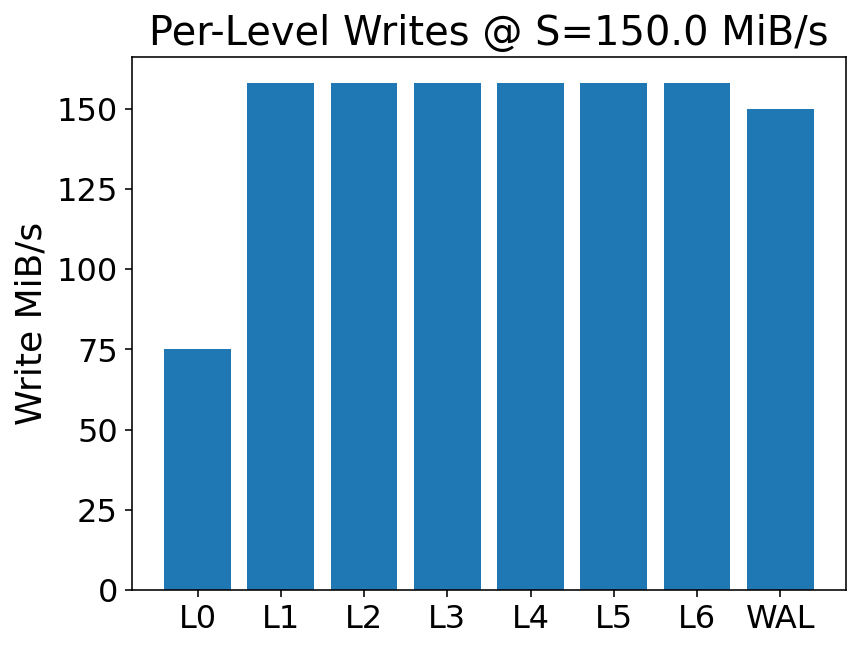
\includegraphics[width=.9\linewidth]{figs/per_level_writes.png}}{\fbox{\parbox{.9\linewidth}{\centering per\_level\_writes.png not found}}}
    \caption{레벨별 쓰기 I/O 분해(예시).}
\end{figure}
\begin{figure}[h]
    \centering
    \IfFileExists{figs/per_level_reads.png}{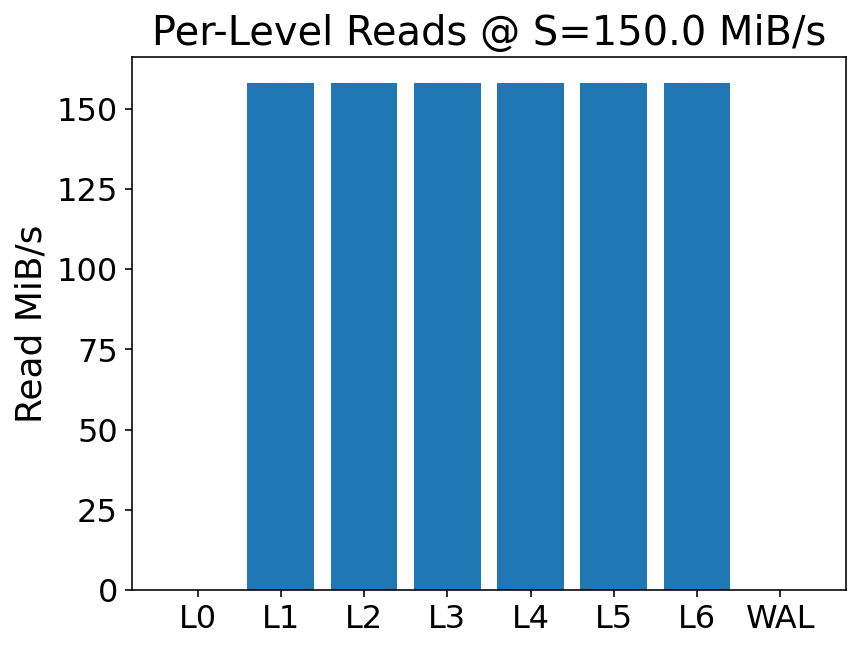
\includegraphics[width=.9\linewidth]{figs/per_level_reads.png}}{\fbox{\parbox{.9\linewidth}{\centering per\_level\_reads.png not found}}}
    \caption{레벨별 읽기 I/O 분해(예시).}
\end{figure}
\begin{figure}[h]
    \centering
    \IfFileExists{figs/depth_summary.png}{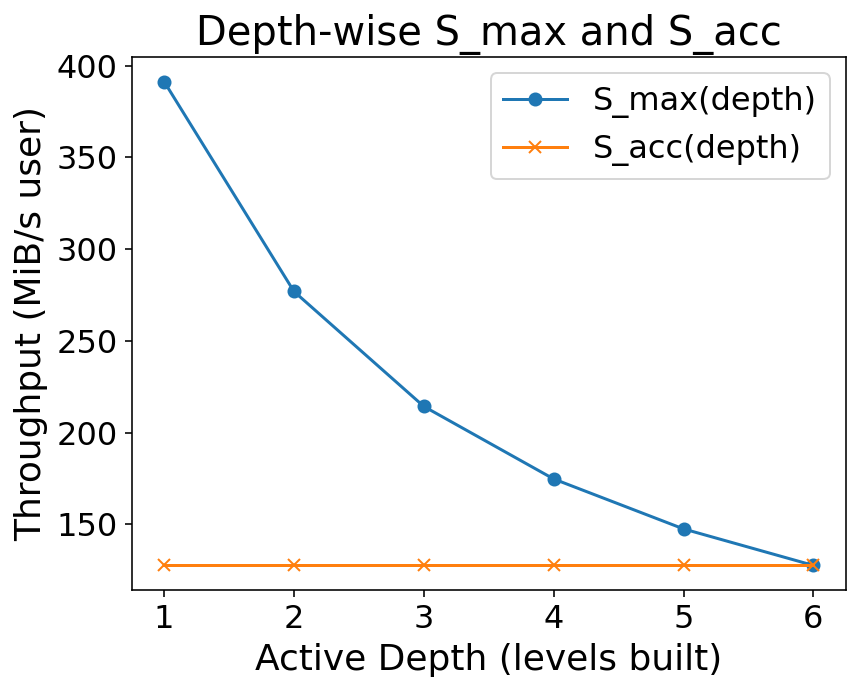
\includegraphics[width=.9\linewidth]{figs/depth_summary.png}}{\fbox{\parbox{.9\linewidth}{\centering depth\_summary.png not found}}}
    \caption{초기 버스트 $\rightarrow$ 정상 전이(예시).}
\end{figure}

\section*{맺음말}
본 재구성 문서는 \texttt{PutModel.html}의 핵심을 식과 절차 중심으로 압축하여,
현장 적용 시의 해석 가능성과 검증 용이성을 높였다.
실제 배포 환경에서는 장치/워크로드 특성에 맞춘 보정(\(CR,WA,RA_c\))과
지속 모니터링을 결합해, \(\,S_{\max}\) 운영 엔벨롭 안에서 안정적 성능을 확보하기를 권장한다.

\end{document}
